\documentclass[12pt,oneside,a4paper]{article}
\usepackage{fancyhdr}
\newlength\tindent
\setlength{\tindent}{\parindent}
\setlength{\parindent}{0pt}
\renewcommand{\indent}{\hspace*{\tindent}}
\usepackage{parskip}
\usepackage{nicefrac}
\usepackage{algorithm}
\usepackage{algpseudocode}
% for the codes
\usepackage{listings}
\usepackage{xcolor}
\definecolor{codegreen}{rgb}{0,0.6,0}
\definecolor{codegray}{rgb}{0.5,0.5,0.5}
\definecolor{codepurple}{rgb}{0.58,0,0.82}
\definecolor{backcolour}{rgb}{0.95,0.95,0.92}
 
\lstdefinestyle{mystyle}{
    backgroundcolor=\color{backcolour},   
    commentstyle=\color{codegreen},
    keywordstyle=\color{magenta},
    numberstyle=\tiny\color{codegray},
    stringstyle=\color{codepurple},
    basicstyle=\footnotesize,
    breakatwhitespace=false,         
    breaklines=true,                 
    captionpos=b,                    
    keepspaces=true,                 
    numbers=left,                    
    numbersep=5pt,                  
    showspaces=false,                
    showstringspaces=false,
    showtabs=false,                  
    tabsize=2
}
 
\lstset{style=mystyle}

% some very useful LaTeX packages include:

%\usepackage{cite}      % Written by Donald Arseneau
                        % V1.6 and later of IEEEtran pre-defines the format
                        % of the cite.sty package \cite{} output to follow
                        % that of IEEE. Loading the cite package will
                        % result in citation numbers being automatically
                        % sorted and properly "ranged". i.e.,
                        % [1], [9], [2], [7], [5], [6]
                        % (without using cite.sty)
                        % will become:
                        % [1], [2], [5]--[7], [9] (using cite.sty)
                        % cite.sty's \cite will automatically add leading
                        % space, if needed. Use cite.sty's noadjust option
                        % (cite.sty V3.8 and later) if you want to turn this
                        % off. cite.sty is already installed on most LaTeX
                        % systems. The latest version can be obtained at:
                        % http://www.ctan.org/tex-archive/macros/latex/contrib/supported/cite/

\usepackage{graphicx}   % Written by David Carlisle and Sebastian Rahtz
                        % Required if you want graphics, photos, etc.
                        % graphicx.sty is already installed on most LaTeX
                        % systems. The latest version and documentation can
                        % be obtained at:
                        % http://www.ctan.org/tex-archive/macros/latex/required/graphics/
                        % Another good source of documentation is "Using
                        % Imported Graphics in LaTeX2e" by Keith Reckdahl
                        % which can be found as esplatex.ps and epslatex.pdf
                        % at: http://www.ctan.org/tex-archive/info/

%\usepackage{psfrag}    % Written by Craig Barratt, Michael C. Grant,
                        % and David Carlisle
                        % This package allows you to substitute LaTeX
                        % commands for text in imported EPS graphic files.
                        % In this way, LaTeX symbols can be placed into
                        % graphics that have been generated by other
                        % applications. You must use latex->dvips->ps2pdf
                        % workflow (not direct pdf output from pdflatex) if
                        % you wish to use this capability because it works
                        % via some PostScript tricks. Alternatively, the
                        % graphics could be processed as separate files via
                        % psfrag and dvips, then converted to PDF for
                        % inclusion in the main file which uses pdflatex.
                        % Docs are in "The PSfrag System" by Michael C. Grant
                        % and David Carlisle. There is also some information
                        % about using psfrag in "Using Imported Graphics in
                        % LaTeX2e" by Keith Reckdahl which documents the
                        % graphicx package (see above). The psfrag package
                        % and documentation can be obtained at:
                        % http://www.ctan.org/tex-archive/macros/latex/contrib/supported/psfrag/

\usepackage{subfigure} % Written by Steven Douglas Cochran
                        % This package makes it easy to put subfigures
                        % in your figures. i.e., "figure 1a and 1b"
                        % Docs are in "Using Imported Graphics in LaTeX2e"
                        % by Keith Reckdahl which also documents the graphicx
                        % package (see above). subfigure.sty is already
                        % installed on most LaTeX systems. The latest version
                        % and documentation can be obtained at:
                        % http://www.ctan.org/tex-archive/macros/latex/contrib/supported/subfigure/

\usepackage{url}        % Written by Donald Arseneau
                        % Provides better support for handling and breaking
                        % URLs. url.sty is already installed on most LaTeX
                        % systems. The latest version can be obtained at:
                        % http://www.ctan.org/tex-archive/macros/latex/contrib/other/misc/
                        % Read the url.sty source comments for usage information.

%\usepackage{stfloats}  % Written by Sigitas Tolusis
                        % Gives LaTeX2e the ability to do double column
                        % floats at the bottom of the page as well as the top.
                        % (e.g., "\begin{figure*}[!b]" is not normally
                        % possible in LaTeX2e). This is an invasive package
                        % which rewrites many portions of the LaTeX2e output
                        % routines. It may not work with other packages that
                        % modify the LaTeX2e output routine and/or with other
                        % versions of LaTeX. The latest version and
                        % documentation can be obtained at:
                        % http://www.ctan.org/tex-archive/macros/latex/contrib/supported/sttools/
                        % Documentation is contained in the stfloats.sty
                        % comments as well as in the presfull.pdf file.
                        % Do not use the stfloats baselinefloat ability as
                        % IEEE does not allow \baselineskip to stretch.
                        % Authors submitting work to the IEEE should note
                        % that IEEE rarely uses double column equations and
                        % that authors should try to avoid such use.
                        % Do not be tempted to use the cuted.sty or
                        % midfloat.sty package (by the same author) as IEEE
                        % does not format its papers in such ways.

\usepackage{amsmath}    % From the American Mathematical Society
                        % A popular package that provides many helpful commands
                        % for dealing with mathematics. Note that the AMSmath
                        % package sets \interdisplaylinepenalty to 10000 thus
                        % preventing page breaks from occurring within multiline
                        % equations. Use:
%\interdisplaylinepenalty=2500
                        % after loading amsmath to restore such page breaks
                        % as IEEEtran.cls normally does. amsmath.sty is already
                        % installed on most LaTeX systems. The latest version
                        % and documentation can be obtained at:
                        % http://www.ctan.org/tex-archive/macros/latex/required/amslatex/math/

\usepackage{fourier}

% Other popular packages for formatting tables and equations include:

%\usepackage{array}
% Frank Mittelbach's and David Carlisle's array.sty which improves the
% LaTeX2e array and tabular environments to provide better appearances and
% additional user controls. array.sty is already installed on most systems.
% The latest version and documentation can be obtained at:
% http://www.ctan.org/tex-archive/macros/latex/required/tools/

% V1.6 of IEEEtran contains the IEEEeqnarray family of commands that can
% be used to generate multiline equations as well as matrices, tables, etc.

% Also of notable interest:
% Scott Pakin's eqparbox package for creating (automatically sized) equal
% width boxes. Available:
% http://www.ctan.org/tex-archive/macros/latex/contrib/supported/eqparbox/

% *** Do not adjust lengths that control margins, column widths, etc. ***
% *** Do not use packages that alter fonts (such as pslatex).         ***
% There should be no need to do such things with IEEEtran.cls V1.6 and later
\pagestyle{fancy}
%\fancyhf{}
\fancyhead[LE,RO]{HPP Course -- Assignment 5 -- Group 55}
%\fancyhead[LO,RE]{Student: \textbf{Tuan Anh Dao}}
\fancypagestyle{firststyle}
{
   \fancyhf{}
   \fancyfoot[C]{\footnotesize Page \thepage\ of \pageref{LastPage}}
}

% Your document starts here!
\begin{document}
% Define document title and author
	\title{High Performance Programming Report\\[0.5cm]
		\large{Assignment 5: Solving the N-body problem\\using Barnes-Hut method with parallelization}
	}
	\author{Group 55: \hspace{1cm} \textit{Peralta Alguacil, Francisco Jose}\\ \textit{Dao, Tuan Anh}}
	%\thanks{Lecturer.}}
	%\markboth{Applied Finite Element Method (Autumn 2017)}{}
	\maketitle
	\pagestyle{fancy}

\section{Introduction}
\label{sec:intro}
In this assignment, we study the N-body problem under the view of Newton's law of gravitation using Barnes-Hut method with parallelization in the most time-consuming part of the program.

The report is organized as follows: Section \ref{sec:problem} briefly describes the problem; Section \ref{sec:algorithm} discusses the final data structures and algorithms; the choice of $\theta_{\max}$ for the given target accuracy, complexity, performance and related experiments are included in Section \ref{sec:optimization}; Section \ref{sec:conclusion} is the conclusion.

Regarding group collaboration, following previous works, we continued to do programming separately at first. Then we sat together to choose the best implementation on each part. We also based this report on those selections and improvements. We have been using a private \textsc{github.com} repository to manage the code and report files.

\begin{table}[h]
\centering
\caption{CPUs used for performance testing in this report}
\label{tab:cpus}
\hspace*{-1.2cm}
\scalebox{0.8}{
\begin{tabular}{|l|l|l|l|l|}
\hline
\# & \textbf{Name} & \textbf{CPU information} & \textbf{Operating System} & \textbf{Compiler} \\ \hline
1 & Macbook 2016 & Intel(R) Core(TM) i5-6360U CPU @ 2.00GHz & MacOS 10.13.1 & gcc 7.2.0\_1 \\ \hline
2 & Berzelius & Intel(R) Xeon(R) CPU E5520 @ 2.27GHz & Ubuntu 16.04.3 LTS & gcc 5.4.0 \\ \hline
3 & Tussilago  & AMD Opteron(TM) Processor 6282 SE @ 2.60GHz & Scientific Linux 6.9&  2.60GHz, gcc 4.4.7 \\ \hline
\end{tabular}}
\end{table}

In the purpose of reproducibility, we include the information of CPUs in Table \ref{tab:cpus}. From this point on, those machines are well-defined and to avoid duplication, we only cite the names whenever needed.
\section{The N-body problem}
\label{sec:problem}
We shortly recall the N-body problem in this section.

Let $P = \{ p_i \}_{i=1}^N$ be the set of $N$ particles. The following variables are given at time $t_0 = 0$.

\begin{itemize}
\item Let $x_i\in \mathbb{R}^2, i = 1,\dots,N$ be the two-dimensional coordination of particle $p_i$;
\item Let $u_i\in \mathbb{R}^2, i = 1,\dots,N$ be the two-dimensional velocity of particle $p_i$;
\item Let $m_i\in \mathbb{R}, i = 1,\dots,N$ be the mass of particle $p_i$.
\end{itemize}

The objective of this problem is to determine $x_i$, $u_i$ at some desired future time point $t_{k+1} > t_0$.
 
We can solve this problem using \textit{symplectic Euler} -- a finite difference method. By considering an axe of discrete equidistant time points $\{ t_k \}_{k=0}^\infty$ with time step $\Delta t$, we continuously update the values of $x_i, u_i, i=1,\dots,N$ at time $t_{k+1}$ based on the known information at time $t_k$. For this purpose, we define some additional variables at some given time point.

\begin{itemize}
\item Let $F_i\in \mathbb{R}^2, i = 1,\dots,N$ be the two-dimensional force on particle $p_i$;
\item Let $a_i\in \mathbb{R}^2, i = 1,\dots,N$ be the two-dimensional acceleration of particle $p_i$.
\end{itemize}

The new values at time point $t_{k+1}$ are calculated for each particle $i$ as follows.
\begin{enumerate}
\item $\displaystyle F_i^k = -G m_i \sum_{j=1, j\neq i}^N \dfrac{m_j}{(||x_i^k - x_j^k||+\varepsilon_0)^3} (x_i^k - x_j^k)$;
\item $a_i^k = \dfrac{F_i^{k}}{m_i}$;
\item $u_i^{k+1} = u_i^{k} + \Delta t a_i^{k}$;
\item $x_i^{k+1} = x_i^{k} + \Delta t u_i^{k+1}$
\end{enumerate}
where $||.||$ is the normal Euclid norm, $G$ is the gravitational constant and $\varepsilon_0$ is some small real number added to avoid the case when $||x_i - x_j||$ is too small. Throughout this assignment, we use fixed values of constants: $\varepsilon_0 = 10^{-3}, \Delta t = 10^{-5}$ and $G = 100/N$.

However, in the program implementation, by observation, we can avoid redundant calculation in some steps. This point is discussed more in the next section.
\section{Data Structures and Algorithms}
The code is implemented on C language. This section discusses the structure of our program regarding both data and algorithms.
\label{sec:algorithm}
\subsection{Data Structures}

We formed some structs for the ease of managing quadrangles and particles.

\begin{table}[h]
\centering
\caption{Struct \textbf{vector} - common 2D Vector}
\label{tab:struct_vector}
\scalebox{1}{
\begin{tabular}{l|l|l}
\hline
DATA TYPE & NAME & DESCRIPTION \\ \hline \hline
double & x & first coordination of the vector \\ \hline
double & y & second coordination of the vector \\ \hline
\end{tabular}}
\end{table}

\begin{table}[h]
\centering
\caption{Struct \textbf{particle} - coordinations and mass of a particle}
\label{tab:struct_particle}
\scalebox{1}{
\begin{tabular}{l|l|l}
\hline
DATA TYPE & NAME & DESCRIPTION \\ \hline \hline
double & x & first coordination of the particle \\ \hline
double & y & second coordination of the particle \\ \hline
double & m & mass of the particle\\ \hline
\end{tabular}}
\end{table}

\begin{table}[h]
\centering
\caption{Struct \textbf{quadrangle} - a quadrangle object}
\label{tab:struct_quadrangle}
\hspace*{-0.7cm}
\scalebox{1}{
\begin{tabular}{l|l|l}
\hline
DATA TYPE & NAME & DESCRIPTION \\ \hline \hline
double & boundary\_x & x-coordination of the lowest leftmost point \\ \hline
double & boundary\_y & y-coordination of the lowest leftmost point\\ \hline
double & boundary\_length & length of an edge\\ \hline
double & mass & total mass of particles inside it\\ \hline
double & mass\_x & x--coordination of center of mass\\ \hline
double & mass\_y & y--coordination of center of mass\\ \hline
struct particle* & particle & the pointer of particle \\
& & if it contains exactly one (leaf node)\\ \hline
struct quadrangle* & sw & South West child quadrangle\\ \hline
struct quadrangle* & se & South East child quadrangle\\ \hline
struct quadrangle* & ne & North East child quadrangle\\ \hline
struct quadrangle* & nw & North West child quadrangle\\ \hline
\end{tabular}}
\end{table}

As can be seen on the Table \ref{tab:struct_particle}, we only load the coordinations and mass of each particle into the struct. We avoid adding velocity and brightness by storing them in separate arrays of built-in doubles since brightness is not used at all in the iterations, and we only have to update the velocity once after \textit{nsteps} loops. This decreases the size of the struct, and chance is the cache will contains frequently-accessed data for improving the performance.

We could simply use some arrays of doubles instead if we do not need a struct of quadrangle of which properties are included in Table \ref{tab:struct_quadrangle}. This struct is slightly more complicated and is designed to make the idea of quadtree work. Basically, we store some information to determine the position, size and mass distribution of each quadrangle, with four pointers to its four children.
\subsection{Algorithms}
\label{sec:algo}
Since the most problematic part of this assignment is to implement the quadtree correctly, with some operators: insert a new particle, calculate the masses and centers of mass for each nodes of the quadtree, and calculate force using such information of the quadtree, with a parameter of desired accuracy $\theta_{\max}$. We first describe the idea of the main program in Algorithm \ref{algo:main}, then the details of related functions are later explained.

\begin{algorithm}
\caption{Main}\label{algo:main}
\begin{algorithmic}[1]
\Procedure{Main}{}
\State {Load \textit{particles} $\leftarrow$ INPUT}
\For {each time step}
	\State {Initialize the quadtree}
	\For {$i=1$ to $N$}
		\State {\textsc{Insert}($i^{th}$ particle) into the quadtree}
	\EndFor
	\State {\textsc{CalculateMass}(quadrangles) for all nodes of the quadtree}
	\For {$i=1$ to $N$}
		\State {\textsc{CalculateForce}($i^{th}$ particle)}
	\EndFor
	\State {Update the new values of coordinations for all particles}
	\State {Deallocate the quadtree}
\EndFor
\State {OUTPUT $\leftarrow$ \textit{particles}}
\EndProcedure
\end{algorithmic}
\end{algorithm}

For the purpose of experimenting, we developed two versions of the same function to insert a new particle into the quadtree. The first one is the recursive version, which described in Algorithm \ref{algo:insert1}. Algorithm \ref{algo:insert2} is the iterative version. Both result same output. Aspects concerning performance and memory usage is more discussed in Section \ref{sec:experiment}. Here we note that only the quadrangles which contain at least one particle is stored. Thus, every leaf node (which does not have children) contains a particle, and a particle is always stored in a leaf node.

\begin{algorithm}
\caption{Insert (Recursive version)}\label{algo:insert1}
\begin{algorithmic}[1]
\Procedure{Insert}{\textit{quadrangle} $n$, \textit{particle} $p$}
	\If {$n$ is NULL}
		\State {Create a new node at $n$ and store $p$ in $n$}
	\ElsIf {$n$ has children}
		\State {Determine the child $m\in \{ sw, se, ne, nw \}$ to which $p$ belongs}
		\State {\textsc{Insert}(m, p)}
	\Else
		\State {\textit{np} $\leftarrow$ (pointer) the particle which $n$ contains}
		\State {Determine the child $m_1\in \{ sw, se, ne, nw \}$ to which \textit{np} belongs}
		\State {Insert a new node at $m_1$ and move \textit{np} to $m_1$}
		\State {Determine the child $m_2\in \{ sw, se, ne, nw \}$ to which \textit{p} belongs}
		\State {\textsc{Insert}($m_2$, p)}
	\EndIf
		
\EndProcedure
\end{algorithmic}
\end{algorithm}

\begin{algorithm}
\caption{Insert (Iterative version)}\label{algo:insert2}
\begin{algorithmic}[1]
\Procedure{Insert}{\textit{quadrangle} $n$, \textit{particle} $p$}
	\If {$n$ is NULL}
		\State {Create a new node at $n$ and store $p$ in $n$}
	\Else
		\State {Find \textit{current} $\leftarrow$ the smallest (can be null) quadrangle containing $p$}
		\State{(this quadrangle contains at most one particle other than $p$)}
		\While {\textit{current} contains another quadrangle \textit{np}}
			\State {Determine and add the children $m_1, m_2\in \{ sw, se, ne, nw \}$}
			\State {to which \textit{np}, $p$ belongs, respectively;}
			\State {current $\leftarrow m2$}
		\EndWhile
	\EndIf
\EndProcedure
\end{algorithmic}
\end{algorithm}

Next algorithm recursively calculates the mass of each node in the quadtree.

\begin{algorithm}
\caption{Calculate Mass}\label{algo:mass}
\begin{algorithmic}[1]
\Procedure{CalculateMass}{\textit{quadrangle} $n$}
	\If {n is a leaf node}
		\State {$n$ surely contains a particle $p$}
		\State {$n$.mass $\leftarrow$ $p$.mass;}
		\State {center of mass of $n$ $\leftarrow$ coordinates of $p$;}
	\Else
		\State {mass $\leftarrow$ 0; center\_of\_mass = 0;}
		\For {each child $m$ of $n$}
			\State {mass\_m $\leftarrow$ \textsc{CalculateMass}($m$);}
			\State {mass $\leftarrow$ mass + mass\_m;}
			\State {center\_of\_mass $\leftarrow$ center\_of\_mass + mass * $m$.center\_of\_mass;}
		\EndFor
		\State {center\_of\_mass $\leftarrow$ center\_of\_mass / mass;}
	\EndIf
\EndProcedure
\end{algorithmic}
\end{algorithm}

Algorithm \ref{algo:force} recursively calculates the force on each particle caused by all particles inside a quadrangle $n$ in the quadtree.

\begin{algorithm}
\caption{Calculate Force}\label{algo:force}
\begin{algorithmic}[1]
\Procedure{CalculateForce}{\textit{quadrangle} $n$, particle $p$}
	\State {$\theta = \dfrac{\text{$n$.boundary\_width}}{||\text{$n$.center\_of\_mass - $p$.coordinates}||_{\text{Euclid}}}$;}
	\If {$n$ is a leaf node OR $\theta < \theta_{\max}$}
		\State {Calculate the force between $n$ and $p$ as in Section \ref{sec:problem}}
	\Else
		\State {total\_force $\leftarrow$ 0}
		\For {each child $m$ of $n$}
			\State {total\_force $\leftarrow$ total\_force + \textsc{CalculateForce}($m$, $p$)}
		\EndFor
	\EndIf
\EndProcedure
\end{algorithmic}
\end{algorithm}

Alternative options on data structures and algorithms:

\begin{itemize}
\item \textbf{Storing all the data on separate arrays}. It is possible if we use a straightforward $\mathcal{O}(N^2)$ algorithm. However, in this assignment, since the structure of quadtree is used, it is much more convenient for the operations on quadtree to store some properties of the particles in another struct.
\item \textbf{Full struct of particle: we could use a full struct of the particle}. However, for the purpose of caching, we only want to call the most frequently-accessed properties, which are coordinates and mass. Properties like brightness are even not used in the computation; and we only have to update the velocity once at the last iteration.
\item \textbf{Recursive or Iterative function?} If implemented correctly, the time complexity is the same for both implementations. However, if the size of the problem is really large, then it is necessary to avoid the recursive functions since it will use a huge amount of stack memory and it could lead to a stack overflow. However, in this assignment, because of the size of the problem, it is possible to use the recursive version since it is much easier to understand. We did both implementations and give some comparisons in Section \ref{sec:experiment}.
\end{itemize}

\section{Experiments, Optimizations and Complexity}
\label{sec:experiment}
The content in this section involves some performance results in real time measurements. The time (wall) was measured using the same function \textit{get\_wall\_seconds()} as in the lab. The total time includes both I/O time and calculation time.

\label{sec:optimization}
\subsection{Choice of $\theta_{\max}$ for the given target accuracy}
Since the suggestion of $\theta_{\max}$, we calculated the pos\_maxdiff with different values of $\theta_{\max}$ between $[0.02, 0.5]$. Intuitively, the larger $\theta_{\max}$ is, the bigger error (or pos\_maxdiff) will be. Thus, the line graph in Figure \ref{fig:theta_max} should be monotonously increasing. Therefore, we draw a red line of error threshold to illustrate the maximum tolerance for pos\_maxdiff. The maximum value of $\theta_{\max}$ satisfying the target accuracy we found is \textbf{0.256}. We could have found more precise value but we decided to stop there.

\begin{figure}[h]
	\centering
	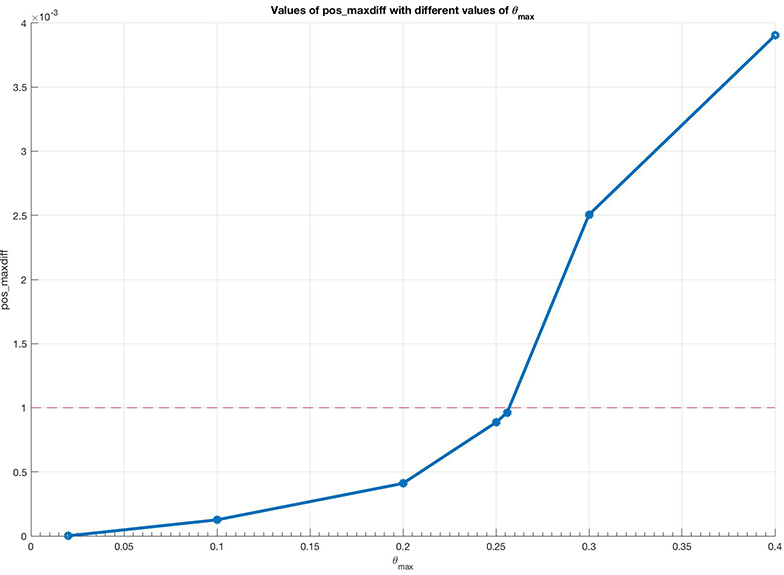
\includegraphics[scale=0.5]{theta_max.jpg}
	\caption{Values of pos\_maxdiff resulted by different values of $\theta_{\max}$}
	\label{fig:theta_max}
\end{figure}

\subsection{Final results}

The wall time was measured using the \textbf{time} command. Each result is the best time among five trials. We did these performance testings on Macbook 2016 and Berzelius of which information was stated in Section \ref{sec:intro}.

\begin{table}[h]
\centering
\caption{Final performance results with different optimization flags (in seconds)}
\label{tab:struct_particle}
\scalebox{1}{
\begin{tabular}{|l|ll|ll|}
\hline
Optimization flag & \textbf{Macbook 2016} & Speedup & \textbf{Berzelius} & Speedup \\ \hline \hline
No flag & 8.34s & 1 & 14.89s & 1 \\ \hline
\textsc{-O2} & 3.94s & 2.12 & 6.97s & 2.14\\ \hline
\textsc{-O3} & 3.91s & 2.13 & 6.97s & 2.14\\ \hline
\textsc{-O3} \textit{-march=native -ffast-math} & 3.93s & 2.12 & 6.67s & 2.23\\ \hline
\end{tabular}}
\end{table}

We can observe that adding flags has significant improvement in the performance of the program. However, the results for \textsc{-O2} and \textsc{-O3} flags are quite similar in both machines. For \textbf{Macbook 2016}, the \textit{-march=native -ffast-math} flag does not make any improvement in comparison with \textsc{-O3} but it does in the other one \textbf{Berzelius}. We also include speedup results along with the time results to illustrate the efficiency.

\subsection{Experiments}

\subsubsection{Replacing recursive functions by iterative functions}
-Same time complexity

-Better space complexity (use memcheck valgrind)

-Avoid stack overflow

\subsubsection{Complexity of each operator on the quad tree}

\subsection{Program complexity}
The performance measurements in this section were done on \textbf{Berzelius} with \textsc{-O3} optimization flag. Table \ref{tab:complex_1} indicates the computation time for sets with different number of particles. We got the time in cases $\theta_{\max} = 0$ for $\mathcal{O} (N^2)$ complexity, and $\theta_{\max} = 0.256$. The time was measured by placing the \textbf{get\_wall\_seconds()} which is similar to the one in the lab, at the beginning and the end of the program, except the I/O procedures. This is because on our server \textbf{Berzelius}, the I/O time is really random and it does not make sense if we include those to evaluate the complexity. The slots marked with "--" are bigger than 100s. We also plotted the computation time versus the number of particles for checking the real complexity in Figure \ref{}.

\begin{table}[h]
\centering
\caption{Computation time on \textbf{Berzelius} with different values of $N$}
\label{tab:complex_1}
\scalebox{1}{
\begin{tabular}{l|l|l}
\hline
N & Wall time with $\theta_{\max} = 0.256$ & Wall time with $\theta_{\max} = 0$ \\ \hline \hline
10 & 0.0009370 & 0.0010390\\ \hline
20 & 0.0031040 & 0.0035601\\ \hline
30 & 0.0089421 & 0.0069938\\ \hline
40 & 0.0110779 & 0.0115230\\ \hline
50 & 0.0173981 & 0.0178390\\ \hline
60 & 0.0223758 & 0.0280061\\ \hline
70 & 0.0287378 & 0.0335340\\ \hline
80 & 0.0335600 & 0.0423331\\ \hline
90 & 0.0392060 & 0.0534279\\ \hline
100 & 0.0442431 & 0.0651462\\ \hline
150 & 0.0805900 & 0.1430421\\ \hline
200 & 0.1214850 & 0.2762249\\ \hline
300 & 0.2295508 & 0.6667540\\ \hline
400 & 0.3666220 & 1.1795640\\ \hline
500 & 0.5067809 & 1.8718028\\ \hline
600 & 0.6812260 & 2.6995649\\ \hline
700 & 0.8349972 & 3.8379309\\ \hline
800 & 1.0206718 & 4.8004501\\ \hline
900 & 1.1958830 & 6.1728532\\ \hline
1000 & 1.4003611 & 7.8991399\\ \hline
2000 & 3.7918429 & 40.7159750\\ \hline
3000 & 6.8999462 & 97.6599860\\ \hline
4000 & 10.1695912 & --\\ \hline
5000 & 13.6909249 & --\\ \hline
6000 & 17.2950299 & --\\ \hline
7000 & 21.1669080 & --\\ \hline
8000 & 25.2523329 & --\\ \hline
9000 & 29.6465890 & --\\ \hline
\end{tabular}}
\end{table}

\begin{figure}[h]
	\centering
	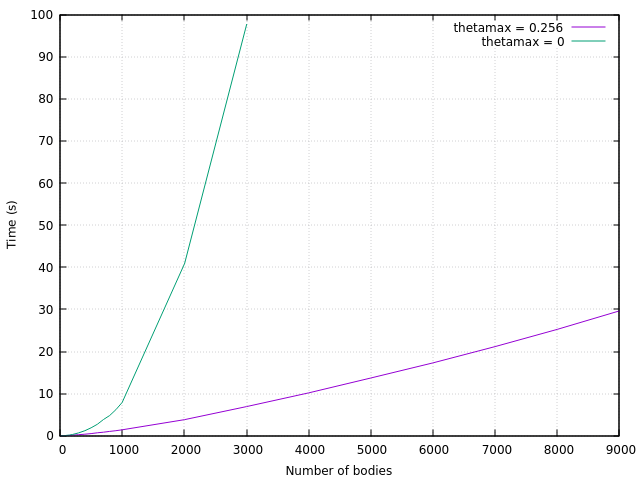
\includegraphics[scale=0.9]{complexity.png}
	\caption{complexity}
	\label{fig:complexity}
\end{figure}

As can be seen from Figure \ref{fig:complexity}, when setting $\theta_{\max} = 0.256$ (Barnes-Hut implementation), we obtain the expected $\mathcal{O} (N\log(N))$ complexity while in case $\theta_{\max} = 0$, we have the shape of $\mathcal{O} (N^2)$ complexity.



\section{Conclusion}
\label{sec:conclusion}
\end{document}